%\section{Anforderungen}

%Das zu entwickelnde Programm wird online per Java Servlets zur Verfügung gestellt. Als Webserver wird der %Tomcat eingesetzt. Folgende Funktionalitäten sollen umgesetzt weden:

%\begin{itemize}
%\item Loginsystem für Lernenden und Betreuer
%\item Grafische Oberfläche
%\item Eintragen von neuen Übungsaufgaben bestehend aus:
%	\begin{itemize}
%	\item Sachtext /Aufgabenstellung
%	\item Musterlösung(en)
%	\item Angabe von realen Datenbanken mit Testdaten
%	\item Einteilung in Kategorie
%	\end{itemize}
%\item Löschen und Bearbeiten von Übungsaufgaben
%\item Erstellen, Bearbeiten und Löschen von Kategorien
%\item Lösen von Übungsaufgaben durch Angabe einer SQL-Anfrage
%\item Tracking von Lösungsversuchen (Versuch, AufgabenID, Timestamp, UserID)
%\item Tracking von Usern und letzten Aktivitäten
%\item Tracking von Fehlern/ Fehlversuchen pro Aufgabe/User
%\end{itemize}


Im folgendem Abschnitt beschreiben wir die Struktur des Programms und gehen, in übersichtlicher Form, auf die einzelnen Klassen und Funktionen des Programms ein. Eine noch detaillierte Fassung der Dokumentation findet sich im Quelltext als Javadocs-Kommentare.

\section{Datenbankstruktur}

Wir benutzen eine Datenbank um Aufgabenstellungen, Nutzer, Lösungsversuche und vieles mehr abzuspeichern. Im folgenden werden die einzelnen Tabellen erläutert. Wir verwenden dazu bewusst eine abstraktere Form der Beschreibung. Begründet ist dies, durch die Vielfalt der verschiedenen DBMS und ihrer verschiedenen Auslegung der Data Defintion Language. Im Prototypen verwenden wir das DBMS MySQL, man könnte aber alle DBMS verwenden, die einen JDBC Connector haben.

\textbf{attempts} (\underline{id}, userid $\to$ user(id), taskid $\to$ tasks(id), timeat ,sqlstatement ,correct)

Die Tabelle \verb|attempts| speichert je einen Lösungsversuch eines Benutzers. Dabei wird die SQL-Anfrage (\verb|sqlstatement|) eines Benutzers (mit der ID \verb|userid|) mit der Uhrzeit (\verb|timeat|) abgespeichert. Weiterhin wird vermerkt, welche Aufgabe (\verb|taskid|) der Student lösen wollte und, ob dieser Korrekt war.

\textbf{dbschema} (taskid $\to$ tasks(id), name, schema)

In der Tabelle \verb|dbschema| speichern wir zu jeder Aufgabe \verb|taskid|, wie die Struktur der Tabelle dafür aussieht. Wir speichern dazu, möglichst SQL-92 konforme, \verb|CREATE TABLE|-Anweisungen im Attribut \verb|schema|. Wir ordnen dem Schema außerdem einen Namen zu, damit es später einfach wiederzufinden ist.

\textbf{external\_database} (id, uri, dbname, username, password, typ)

Die Tabelle \verb|external_database| speichert die Zugriffsdaten (\verb|username,password|) einer externen Datenbank, die verwendet wird, um die notwendigen Bedingung einer Äquivalenz zu prüfen. Weiterhin speichern wir den Zugriffspfad auf diese Datenbank (\verb|uri|) und den Datenbanknamen (\verb|dbname|). Schließlich speichern wir noch den Typ. Im Moment werden mysql, postgresql und oracle als Typ unterstützt. Wir gehen später darauf ein, wie wir die Funktionalität auf noch mehr Datenbanken ausweiten können.

\textbf{samplesolutions} (id, taskid, sqlstatement)

Die Musterlösung für eine Aufgabe, wird in der Tabelle \verb|samplesolutions| gespeichert. Wir erfassen dabei die Aufgabennummer (\verb|taskid|), sowie die Musterlösung als SQL-Anfrage (\verb|sqlstatement|). Wir verwenden einen künstlichen Schlüssel \verb|id|, da es unter Umständen mehrere Musterlösungen zu einer Aufgabe geben kann.

\textbf{tasks} (id, description, respectColumnOrder, schemaid, createdAt$^0$)

Die Aufgaben werden in der Tabelle \verb|tasks| gespeichert. Wir versehen jede Aufgabe mit einer \verb|id| und einer Beschreibung, in Form eines Sachtextes (\verb|description|). Wir speichern, ob die Reihenfolge der Spalten (im \verb|SELECT|-Teil) eingehalten werden muss und, erfassen außerdem, welches Datenbankschema zu dieser Aufgabe zugeordnet werden soll. Optional können wir noch vermerken, wann die Aufgabe eingetragen wurde.

\textbf{tasks\_db} (taskid $\to$ tasks(id), dbid $\to$ external\_database(id))

Es kann unter Umständen möglich sein, pro Aufgabe mehrere externe Datenbanken anzugeben. Daher speichern wir die Zuordnung einer Datenbank zu einer Aufgabe in der Tabelle \verb|tasks_db|. Hierzu verwenden wir den Fremdschlüssel zur Aufgabentabelle (\verb|taskid|) und den zur externen Datenbank (\verb|dbid|).

\textbf{users} (id, name, password, isDozent)

Einzelne Benutzer werden in der Tabelle \verb|users| erfasst. Neben den üblichen Kontoinformationen, wie \verb|name, password| speichern wir auch, ob der Nutzer ein Dozent ist. Diese Information ist wichtig, um zu entscheiden, ob ein Nutzer auch Aufgaben einpflegen darf.

\section{Programmstruktur}

In diesem Abschnitt werden wir die wichtigsten Klassen und Funktionen auflisten und erläutern. Eine vollständige Dokumentation aller Klassen, ist im Quellcode als Javadocs-Kommentare vorhanden. (TODO: evt Anhang).

Das Programm beinhaltet mehrere Prozesse, die sich aus der Abfolge mehrere Funktionen zusammensetzen. Im Folgenden werden alle wesentlichen Prozesse und deren Zusammensetzung erläutert. Wir gehen dabei auch auf Möglichkeiten zur Anpassung des Programms ein.

\subsubsection{Prozess: Standardisieren einer SQL-Anfrage} 

Wir beschäftigen uns zu erst mit einer der Hauptfunktionen: das Standardisieren einer SQL-Anfrage. Die Klasse \verb|QueryHandler| kümmert sich um das Standardisieren einer SQL-Anfrage. Für jede SQL-Anfrage wird ein separates Objekt dieser Klasse erzeugt. Anschließend importieren wir das, zu Grunde liegende, Datenbankschema in das Objekt. Dies geschieht mit der Methode: \\\verb|boolean createTable(String createTableStatement)|\\
Die Methode erwartet pro Aufruf ein, wenn möglich SQL-92 konformes, \verb|CREATE TABLE|-Statement. Nachdem wir das Datenbankschema eingelesen haben, importieren wir noch die zu standardisierende Anfrage. Dies geschieht mit der Methode:\\\verb|setOriginalStatement(String s)|\\ Das eingegebene Statement wird dann mit Hilfe des ZQL-Parsers eingelesen. Etwaige Fehler beim Parsen werden per Exception an den Nutzer weitergereicht. Mehr dazu im Abschnitt >>Webinterface<<. Wir kopieren das Statement außerdem, so dass wir intern zwei ZQuery-Objekte speichern, zum einen die Originalanfrage im Objekt \textbf{original}, die niemals verändert wird, zum Anderen eine Arbeitskopie im Objekt \textbf{workingCopy}, welche wir dann standardisieren. Nun ist das Datenbankschema eingelesen und die, zu verarbeitende, Anfrage liegt vor. Wir können den Standardisierungsprozess nun starten, mit der Methode: \\\verb|ZQuery[] equalize(boolean respect)|\\ 
Als Eingabeparameter erhält sie die Information, ob die Reihenfolge im \verb|SELECT| respektiert werden soll, oder nicht. Im Abschnitt >>externe Datenbanken<< haben wir bereits darüber diskutiert, dass diese Funktion durchaus interessant sein kann. Weiterhin beobachten wir, dass die Methode nicht eine Anfrage, sondern ein Array von Anfragen zurückliefert. Wir erinnern uns an die Problematik der Selbstverbunde. Dort werden mehrere Permutationen der Tabellen unter \verb|FROM| auf die Anfrage angewandt. Es entstehen dann mehrere Anfragen, die alle semantisch äquivalent sind, aber Aufgrund ihrer unterschiedlichen Struktur alle, mit der Lösung des Lernenden abgeglichen werden müssen.

Die Funktion \verb|equalize| startet die Funktion:\\
\verb|handleQUERY(ZQuery q)|\\Zu beachten ist der Parameter. Da die Abfrage während des Standardisierens verändert wird, ist die ursprüngliche Anfrage des Studenten, unwiederbringlich, verändert. Damit dies nicht geschieht, entscheiden wir nun welche Anfrage zum Standardisieren übergeben wird. Wir übergeben hier das Objekt \textit{workingCopy}.

\verb|handleQUERY| speichert zunächst alle Metainformationen der Anfrage in einem Objekt der Klasse \verb|MetaQueryInfo|. Wie dies genau geschieht behandeln wir später, in diesem Kapitel. Anschließend verarbeitet \verb|handleQUERY| mit Hilfe der Methode:\\
\verb|handleFROM|\\
den \verb|FROM|-Teil unserer Anfrage. Die Verarbeitung hängt vom \verb|SELECT|-Teil ab. Wie bereits in Kapitel \ref{chap:theorie} besprochen, werden, abhängig vom \verb|SELECT|-Teil, die Tabellen zunächst sortiert. Anschließend erhalten alle Tabellen einen künstlichen Alias, der fortlaufend ist. In der Standardeinstellung des Programmes ist dies \verb|a1, a2, a3, ...| Die verwendeten Aliase werden nun in einer \textit{HashMap} als Attribut \textbf{Zuordnung} in der Klasse QueryHandler gespeichert. 

Anschließend bearbeiten wir den \verb|SELECT|-Teil unserer Anfrage mit der Funktion:\\
\verb|Vector<ZSelectItem> handleSELECTClause(Vector<ZSelectItem> sel)|\\
Im wesentlichen ändern wir hier vorhandene Aliase in unsere automatisch erzeugten. Finden wir dabei Attribute, die keine Aliase besitzen und es mehrere Tabellen unter \verb|FROM| gibt, die dieses konkrete Attribut beinhalten, lösen wir eine Fehlermeldung aus, wegen Uneindeutigkeit.

Jetzt erstellen wir Permutationen der Tabellen in der \verb|FROM|-Liste. Wir gehen dabei vor, wie im Kapitel \ref{chap:theorie} beschrieben. Sind in unter \verb|FROM| keine zwei gleichen Tabelle, dann enthält die Menge der Permutationen nur die ursprüngliche Anordnung. Die nun folgenden Schritte werden für jede permutierte \verb|FROM|-Liste durchgeführt.

\verb|equalize| fährt fort mit der Methode: \verb|ZExp handleWHERE(ZExp exp)|.\\
Innerhalb dieser Methode erledigen wir alle Arbeiten, die im Abschnitt >>WHERE-Teil<< in Kapitel \ref{chap:theorie} erläutert wurden. Zunächst führen wir die künstlichen Aliase ein mit der Funktion \verb|makeAlias|. Dies geschieht in ähnlicher Weise, wie im \verb|SELECT|-Teil. \verb|makeAlias| sucht auch nach Unterabfragen. Findet es solche, werden diese ersetzt durch ihre standardisierte Form, indem der Standardisierungsprozess für diese rekursiv aufgerufen wird. Danach transformieren wir, mit der Funktion \verb|transformToKNF|, die aktuelle Form des \verb|WHERE|-Ausdrucks in eine konjunktive Normalform. Dabei bedient sich \verb|transformToKNF| der Funktionen:\\
\verb|operatorCompression, pushDownNegate| und \verb|distribute|. Die Vorgehensweise entspricht der besprochenen im theoretischen Bereich dieser Arbeit. Wir ersetzen danach Unterabfragen durch \verb|EXISTS|-Unterabfragen, wenn möglich. Anschließend werden implizite Formeln hinzugefügt sowie arithmetische und logische Ausdrücke ausgewertet, soweit dies möglich ist. Gerade durch die letzten, beiden Teilschritte, kann es passieren, dass die konjunktive Normalform wieder zerstört worden ist. Daher wenden wir an dieser Stelle erneut \verb|transformToKNF| an. Als letzten Schritt sortieren wir den Ausdruck so, wie ausführlich im Bereich \ref{subsec:sort} beschrieben. Die Sortierung beinhaltet auch die Duplikateliminierung bei doppelten \verb|AND|- oder \verb|OR|-Operanden.

\verb|handleQUERY| wendet sich jetzt dem \verb|GROUP BY|-Teil zu. Dieser wird in zwei Teilen abgearbeitet. ZQL trennt \verb|GROUP BY|- vom \verb|HAVING|-Teil. Im \verb|GROUP BY|-Teil sortieren wir lediglich lexikographisch, wie schon im \verb|SELECT|-Teil. Der \verb|HAVING|-Teil wird mit der Funktion \verb|handleWHERE| behandelt, da sich beide Ausdrücke strukturell gleichen.

Der entstandene SQL-Ausdruck, in Form eines \verb|ZQuery|-Objektes, wird von \verb|handleQUERY| direkt zu \verb|equalize| zurückgeliefert. Der Standardisierungsprozess ist damit beendet. Abbildung \ref{fig:execPlan} soll die Reihenfolge der abgearbeiteten Funktionen noch einmal verdeutlichen. 

\begin{figure}[h]
\centering
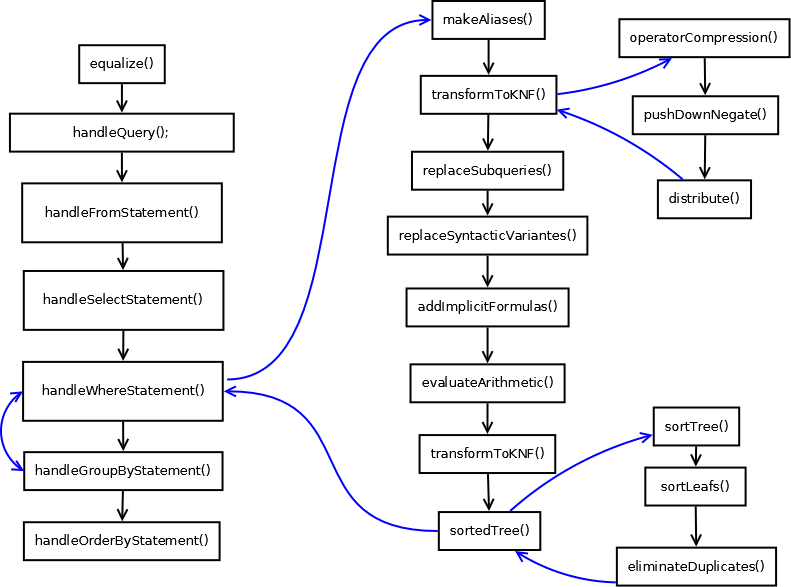
\includegraphics[scale=0.39]{Bilder/execPlan.png}
\caption{Einfacher Programmablaufplan}
\label{fig:execPlan}
\end{figure}

\subsection*{Prozess: Verwenden von externen Datenbanken} 

Nachdem wir den Prozess der Standardisierung ausführlich betrachtet haben, kommen wir nun zum zweiten, großen Prozess. Es handelt sich hierbei um das Ausführen der zwei Anfragen auf externen Datenbanken und dem Vergleich der Ergebnismengen. Hierfür verwenden wir hauptsächlich die Klasse \verb|QueryUtils|, welche eine Sammlung von nützlichen Funktionen zum Behandeln der SQL-Anfragen beinhaltet. Doch zunächst beginnen wir mit dem Ausführen einer SQL-Anfrage auf einer externen Datenbank. Grundsätzlich können zu jeder Aufgabe beliebig viele externe Datenbanken angegeben werden. Die Lösungen würden dann auf allen diesen Datenbanken ausgeführt werden. Dies ist nützlich, um verschiedene Datenbankzustände zu testen. Weiterhin können so Eigenheiten unterschiedlicher DBMS aufgezeigt werden. 

Alle, uns zur Verfügung stehende, externe Datenbanken sind wiederum in unserer internen Datenbank abgespeichert, in Form von ID, Hostname, Port, Datenbankname, Benutzername, Passwort und Typ. Unterstützte Typen sind zur Zeit MySQL, PostgreSQL und Oracle. Allerdings kann die Funktionalität jederzeit erweitert werden. Notwendig ist dazu lediglich das Einpflegen des jeweiligen JDBC-Connectors. Die statische Klasse \verb|externalDB| regelt nun das Ausführen einer eingegebene SQL-Anfrage \verb|q| auf der externen Datenbank mit der ID \verb|dbid|. \\
\verb|static ResultSet executeQueryOn(String q, int dbid)|\\
Die Methode \verb|executeQueryOn| liefert ein \verb|ResultSet| zurück. Dabei extrahiert sie zunächst die Zugangsdaten für die externe Datenbank mit Hilfe der \verb|dbid|. Im zweiten Schritt wird der korrekte JDBC-Connector geladen und eine Datenbankverbindung geöffnet. Nach dem Ausführen der Anfrage \verb|q|, wird die Ergebnismenge in Form eines \verb|ResultSet| zurückgegeben. Möchte man weitere DBMS unterstützen, so müssen in dieser Methode die JDBC-Connector eingepflegt werden.

Wie bereits im Kapitel \ref{chap:theorie} besprochen, entfernen wir ,vor dem Ausführen der Anfragen auf externen Datenbanken, das \verb|ORDER BY|-Statement von der Lösung des Lernenden, wenn die Musterlösung kein solches Statement enthält.

Nach dem Ausführen der Anfragen erhalten wir zwei Objekte vom Typ \verb|ResultSet|, nämlich \verb|r1| und \verb|r2|. Um zu prüfen, ob beide Ergebnismengen identisch sind, bedienen wir uns eine Funktion aus der Klasse \verb|QueryUtils|.\\
\verb|boolean isIdenticalResultSets(ResultSet r1, ResultSet r2)|\\
Die Methode geht recht intuitiv vor. Wir gehen iterativ alle Tupel durch und für jedes Tupel prüfen wir, Schritt für Schritt, ob alle Spalteneinträge identisch sind. Sind Spaltenlängen, Zeilenlängen oder Inhalte der Spalten nicht identisch, so sind beide Ergebnismengen ebenfalls nicht identisch. Die Reihenfolge der Tupel ist vorgegeben durch die \verb|ORDER BY|-Statements beider Anfragen. Die Reihenfolge der Spalten ist vorgegeben durch das \verb|SELECT|-Statement. Bereits im Schritt der Standardisierung wurden die \verb|SELECT|-Einträge sortiert, wenn ausdrücklich in der Aufgabenstellung notiert war, dass die Spaltenreihenfolge keine Rolle spielt. Aus diesen Gründen ist es legitim, die Ergebnismengen in dieser Art zu vergleichen.

\subsection*{Prozess: Auswerten von Metainformationen} 

Im Prozess: Standardisierung haben wir bereits erfahren, dass vor dem Anpassen der SQL-Anfrage, Metainformationen über diese abgespeichert werden. Dazu wird ein Objekt der Klasse \verb|MetaQueryInfo| erstellt. Dem Konstruktor wird die, zu analysierende, SQL-Anfrage in Form eines \verb|ZQuery| übergeben. Mit Hilfe verschiedener Hilfsfunktionen werden dann Informationen über die SQL-Anfrage gesammelt und gespeichert. Beispiele für diese Informationen sind: Anzahl der Verbunde, Größe der \verb|SELECT|-Liste, Anzahl der Tabellen unter \verb|FROM|, Anzahl von Unterabfragen, e.t.c. 

Die Informationen sind einzeln nicht interessant. Nur der Vergleich der Metainformationen von der Musterlösung mit der Lösung des Lernenden, geben Aufschluss über etwaige Fehler. Diesen Vergleich übernimmt eine statische Funktion aus der Klasse \verb|QueryUtils|.\\
\verb|static String compareMetaInfos(MetaQueryInfo m1, MetaQueryInfo m2)|\\
Um die Art des Vergleiches zu verstehen, muss darauf hingewiesen werden, dass alle gespeicherten Attribute in einem Objekt vom Typ \verb|MetaQueryInfo| entweder vom Typ \textbf{int} oder vom Typ \textbf{boolean} sind. Ganzzahlige Attribute verwenden wir um die Anzahl von etwas festzustellen, also \mbox{z. B.} die Anzahl von Formeln im \verb|WHERE|-Teil. Attribute vom Typ \textbf{boolean} benutzen wir, um festzustellen, ob einzelne Teile einer Anfrage existieren oder nicht.

Der Vergleich erfolgt nun automatisch. Die Methode \verb|compareMetaInfos|, geht iterativ alle Attribute der Objekte \verb|m1| und \verb|m2| durch und erzeugt dabei dynamisch eine Hinweismeldung in Form eines \textbf{String}. Ist das jeweilige Attribut ganzzahlig, so wird geprüft ob das von \verb|m1| größer, kleiner oder gleich im Vergleich zu dem von \verb|m2| ist. Ist es nicht gleich, dann wird eine Meldung erzeugt. Bei der erzeugten Meldung erscheint allerdings nicht einfach der Attributsname, da dies zu kryptisch und unverständlich gegenüber einem Nutzer wäre. Stattdessen kennt die Klasse \verb|QueryUtils| ein Wörterbuch, in Form einer \verb|HashMap|. In dieser ist für jedes Attribut ein Ausgabe-String abgespeichert, der für Nutzer verständlicher ist. Ähnlich wird dann auch mit den Attributen verfahren, die vom Typ \textbf{boolean} sind. Das angesprochene Wörterbuch kann später auch dazu verwendet werden, um Ausgaben in mehreren Sprachen umzusetzen.
Ein Auszug aus dem Programmcode ist in Abbildung \ref{fig:comparecode} zu sehen.

\begin{figure}[h]
\lstset{language=Java,tabsize=2}
\begin{lstlisting}
String res = "";
	for (Field f : m1.getClass().getDeclaredFields()) {
		if (f.getType().toString().equals("int")) {
			String word = null;
			if (f.getInt(m1) < f.getInt(m2)) {
				word = messages.get("less");
			} else if (f.getInt(m1) > f.getInt(m2)) {
				word = messages.get("more");
			}
			if (word != null) {
				String x = "There are " + word + " "
					+ messages.get(f.getName()) + " in the "
					+ messages.get("samplesolution") + " (" + f.getInt(m1)
					+ ") than in yours (" + f.getInt(m2) + ").";
				res += x + "<br>";
			}
\end{lstlisting}
\caption{Quellcode zum Vergleich von ganzzahligen Metainformationen}
\label{fig:comparecode}
\end{figure}

\section{Webinterface}

JSP dient dazu, unser Programm dem Nutzer zugänglich zu machen. Im wesentlichen steuert es dabei die, eben erläuterten, Prozesse. Dieser Teil ist nur prototypisch umgesetzt und durchaus beliebig erweiterbar. Die Grundfunktionalität ist allerdings implementiert. Nachdem sich der Nutzer über die \textbf{login.jsp} eingeloggt hat, sieht er auf der Hauptseite eine kleine Übersicht seiner bisherigen Lösungsversuche. Über das Navigationsmenü links, welches mit der \textbf{nav.jsp} realisiert wurden ist, kann der Nutzer nun die Aufgabensammlung einsehen. Nachdem er eine Aufgabe gewählt hat, wird mit der \textbf{task.jsp} die Aufgabenstellung dargestellt.

Zunächst sieht der Nutzer die Aufgabenstellung in Textform. Anschließend sehen wir welche Tabellen uns, für die Lösung der Aufgabe, zur Verfügung stehen. Darunter befindet sich ein Eingabefeld (1), in dem der Nutzer nun seine Lösung in Form einer SQL-Anfrage stellen kann.

Nachdem der Nutzer seine Lösung eingetragen und durch betätigen des \textit{submit}-Knopfes eingereicht hat, werden die Daten per POST-Methode wieder an die task.jsp gesendet. Die Seite wird wieder aufgebaut und nun um mehrere Ausgaben erweitert. Unter dem Textfeld zur Eingabe der Lösung findet der Nutzer nun seine geparste Eingabe (2). Weiterhin stößt die \textbf{task.jsp} den \verb|equalize| Prozess an. Unter der geparsten Eingabe sieht der Nutzer jetzt auch die standardisierte Eingabe (3). Ein Beispiel ist in Abbildung \ref{fig:screen_prog1} dargestellt.

\begin{figure}[h]
\centering
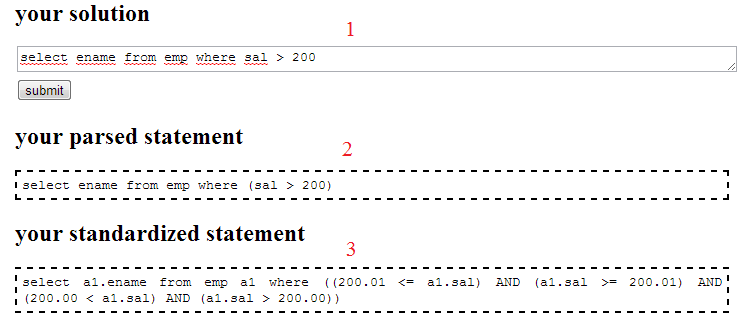
\includegraphics[scale=0.7]{Bilder/screen_prog1}
\caption{Eingabe (1), geparste Eingabe (2) und standardisierte Eingabe (3)}
\label{fig:screen_prog1}
\end{figure}

Nun erstellt die \textbf{task.jsp} drei Blöcke. Im ersten Block (4) sehen wir, ob die standardisierte Musterlösung mit der Lösung des Nutzers gematcht werden konnte. Dazu vergleicht die \textbf{task.jsp} die standardisierte Lösung des Nutzers mit allen standardisierten Lösungen der Musterlösung. Passt eine der standardisierten Musterlösung, so wird dies dem Nutzer mitgeteilt. Falls nicht, so wird darauf hingewiesen, dass dieser Schritt erfolglos war und im nächsten Schritt, die Anfragen auf externen Datenbanken ausgeführt werden.

Im zweiten Block (5) lässt die \textbf{task.jsp} beide Anfragen auf der externen Datenbank ausführen, falls Schritt 1 fehlgeschlagen ist. Wir brauchen hier nicht jede der Musterlösungen ausführen, weil alle das gleiche zurückgeben. Danach werden die Ergebnisse verglichen. Gibt es keine Übereinstimmungen der Ergebnisse, so werden beide Ergebnismengen als Tabellen visualisiert, damit der Nutzer schnell prüfen kann, welche Tupel fehlen oder überflüssig sind. Sind beide Ergebnismengen allerdings identisch, wird dem Nutzer mitgeteilt, das nicht entschieden werden konnte, ob seien Lösung korrekt ist.

Im letzten und dritten Block (6) wird der Vergleich der Metainformationen ausgegeben. Außerdem wird dem Nutzer mitgeteilt, welche Teile seiner Anfrage mit denen der Musterlösung übereinstimmen. Diese Informationen erhält der Nutzer auch wenn bereits Schritt 1 zum Erfolg geführt hat. Mit diesen Informationen sollte es dem Nutzer möglich sein, einen neuen -- hoffentlich erfolgreichen -- Versuch zu starten.

\begin{figure}[h]
\centering
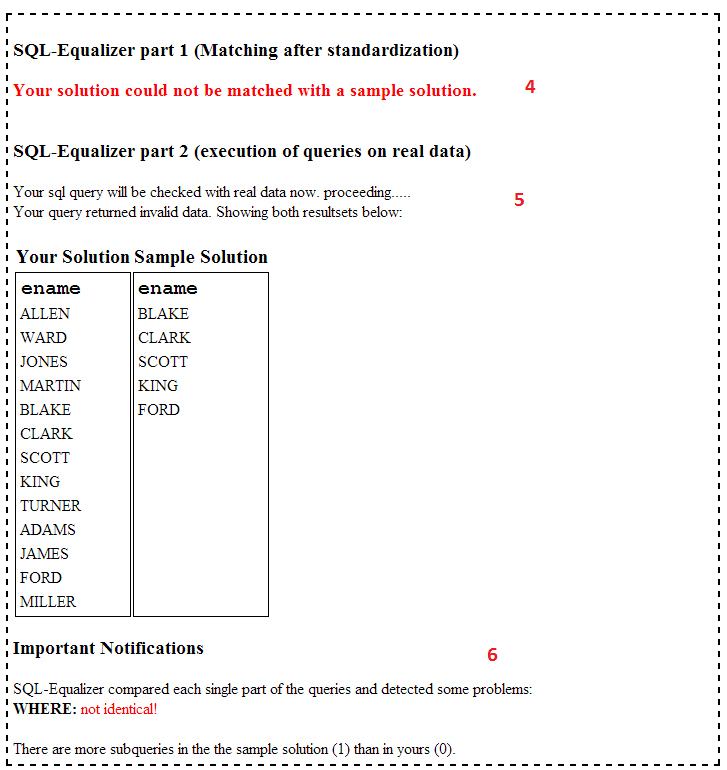
\includegraphics[scale=0.7]{Bilder/screen_prog2}
\caption{Matchingstatus (4), Ergebnistupelvergleich (5) und Hinweise (6)}
\label{fig:screen_prog2}
\end{figure}

Nach all diesen Schritten speichert die \textbf{task.jsp} den Versuch der Lösung in der internen Datenbank ab.

Für Dozenten steht noch die Seite acp.jsp bereit. Hier können neue Datenbankschemata, neue externe Datenbanken, neue Nutzer und neue Aufgabenstellungen eingepflegt werden.
